\subsection{Effective Amplitude and Admissibility Envelope}
  \label{subsec:effective-amplitude-and-admissibility-envelope}

  \begin{definition}
    The effective amplitude of a mode $(\psi_n, a_n)$ is
    \begin{equation}
      A_n := a_n \|\psi_n\|_\infty.
    \end{equation}
    A mode is dynamically admissible in the linearised regime if
    \begin{equation}
      \label{eq:admissibility}
      |\omega_n| \cdot A_n \leq c_\chi.
    \end{equation}
  \end{definition}

  In the linearised dispersion approximation, $\omega_n^2 \approx \lambda_n$, so the
  maximal admissible effective amplitude is
  \begin{equation}
    \label{eq:envelope}
    A_n^{\max} = \frac{c_\chi}{\sqrt{\lambda_n}}.
  \end{equation}
  This defines the admissibility envelope in the $(\lambda_n, A_n)$ plane.

  \begin{figure}[t]
    \centering
    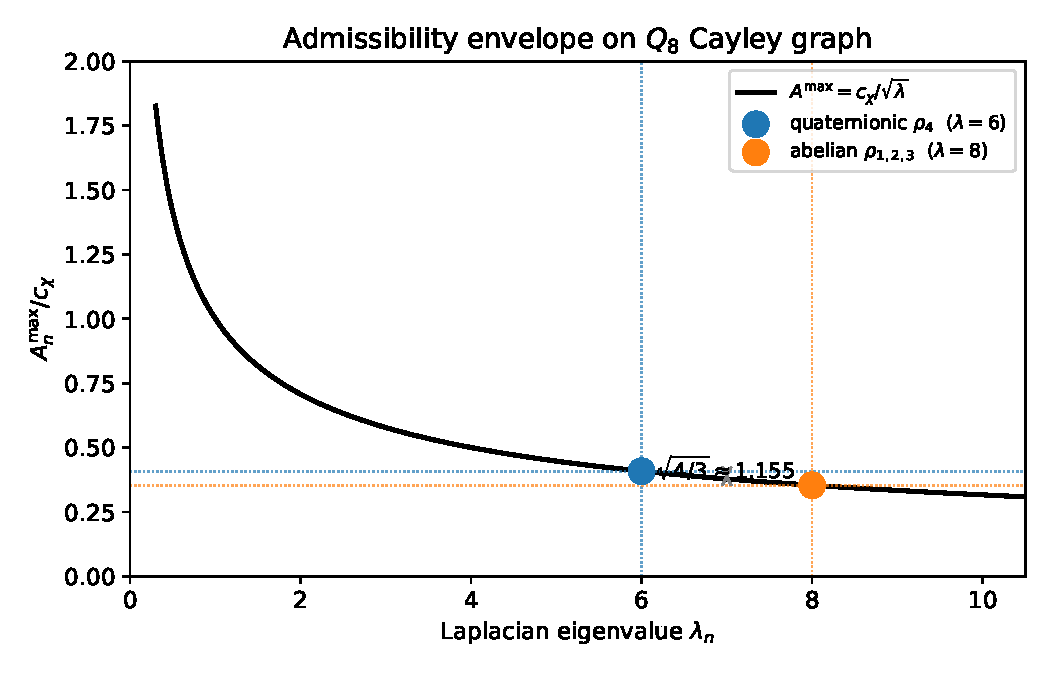
\includegraphics[width=0.82\textwidth]{fig1_Q8_admissibility}
    \caption{
      Admissibility envelope on the $Q_8$ Cayley graph with
      $S=\{\pm i,\pm j,\pm k\}$.
      The maximal effective amplitude
      $A_n^{\max}=c_\chi/\sqrt{\lambda_n}$
      is larger in the quaternionic non-abelian sector
      $\rho_4$ ($\lambda=6$) than in the non-trivial abelian sectors
      ($\lambda=8$), by the factor $\sqrt{4/3}$.
    }
    \label{fig:q8-admissibility}
  \end{figure}

  \begin{remark}
    The linearised dispersion $\omega_n^2 = \lambda_n$ is valid for
    $A_n \ll c_\chi / \sqrt{\lambda_n}$.
    The non-linear Born--Infeld correction modifies this relation near saturation and
    requires a modal reduction of the DBI action.
    The envelope~\eqref{eq:envelope} should therefore be understood first as the
    admissibility boundary in the weakly non-linear regime.
  \end{remark}
